\Appendix{Orientation Move: Mathematical details}
\label{Appendix A}
    In this section, we derive the mathematical formula for the most general case where the bond length is different for image 0, 1 and 2.
    \begin{figure}[!htbp]
        \centering
        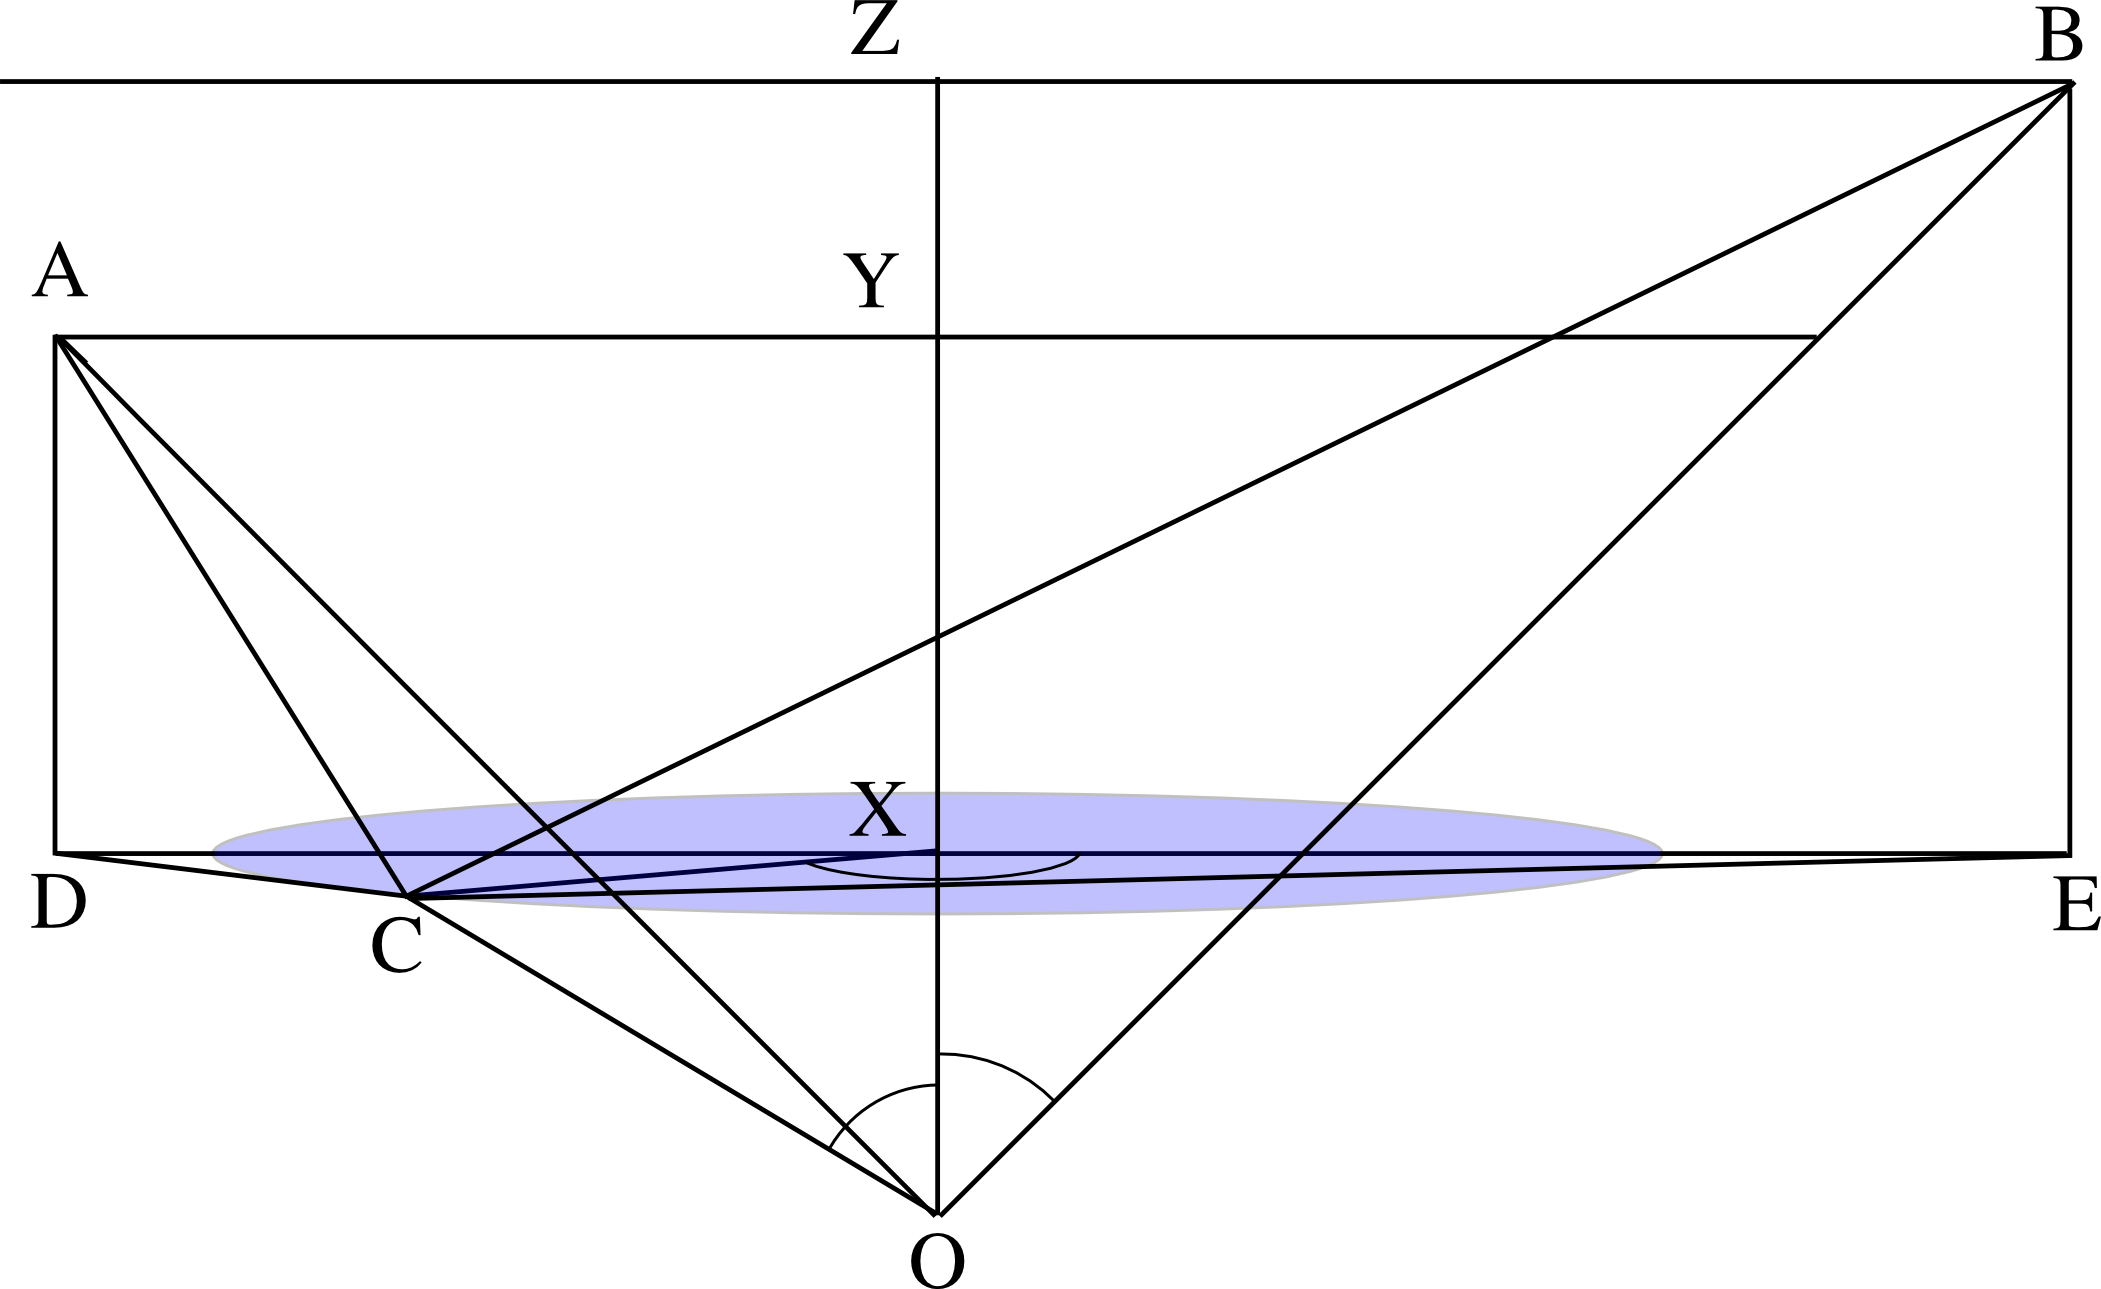
\includegraphics[scale=1.5,keepaspectratio]{Appendix-A/Figures/differentBondlength.png}
        \caption{Simple visualization of the distances involved}
        \label{fig:dist}
    \end{figure}
    Consider the locations of image 0, image 1 and image 2 at A, C and B respectively (see fig. \ref{fig:dist}). All beads and harmonic springs have been omitted from the figure for the sake of clarity. We define the following angles and distances to begin with:
    \begin{itemize}
        \item $\angle AOB = \psi$
        \item $\angle AOX = \angle XOB = \displaystyle\frac{\psi}{2}$
        \item $\angle COX = \alpha$
        \item $\angle CXE = \beta$
        \item $r_0 \equiv d_{OA} = \displaystyle\frac{b_0}{2} , \qquad r_1 \equiv d_{OC} = \frac{b_1}{2}, \qquad r_2 \equiv d_{OB} = \frac{b_2}{2}$
        \item The points O, X, Y and Z are collinear
    \end{itemize}

    In $\Delta AYO ,\angle AOY = \displaystyle\frac{\psi}{2}, \: \: \: \angle AYO = \frac{\pi}{2}$
    \begin{equation}
    \label{eq:ay}
        \Rightarrow d_{AY} = r_0  \sin \Big(\displaystyle\frac{\psi}{2}\Big), \: \: \: d_{OY} = r_0  \cos \Big(\displaystyle\frac{\psi}{2}\Big)
    \end{equation}

    In $\Delta BZO ,\angle BOZ = \displaystyle\frac{\psi}{2}, \: \: \: \angle BZO = \frac{\pi}{2}$
    \begin{equation}
    \label{eq:bz}
        \Rightarrow d_{BZ} = r_2  \sin \Big(\displaystyle\frac{\psi}{2}\Big), \: \: \: d_{OZ} = r_2  \cos \Big(\displaystyle\frac{\psi}{2}\Big)
    \end{equation}

    In $\Delta CXO ,\angle COX = \alpha, \: \: \: \angle CXO = \frac{\pi}{2}$
    \begin{equation}
    \label{eq:cx}
        \Rightarrow d_{XC} = r_1  \sin \big(\alpha\big), \: \: \: d_{OX} = r_1  \cos \big(\alpha\big)
    \end{equation}

    From the figure and eqns. \eqref{eq:ay}, \eqref{eq:bz} and \eqref{eq:cx}, we can clearly see the following:
    \begin{equation}
    \label{eq:adbe}
        \begin{aligned}
            d_{DX} &= d_{AY} = r_0  \sin \Big(\displaystyle\frac{\psi}{2}\Big)\\
            d_{EX} &= d_{BZ} = r_2  \sin \Big(\displaystyle\frac{\psi}{2}\Big)\\
            d_{XY} &= d_{AD} = d_{OY} - d_{OX} = r_0  \cos \Big(\displaystyle\frac{\psi}{2}\Big) - r_1  \cos \big(\alpha\big)\\
            d_{XZ} &= d_{BE} = d_{OZ} - d_{OX} = r_2  \cos \Big(\displaystyle\frac{\psi}{2}\Big) - r_1  \cos \big(\alpha\big)
        \end{aligned}
    \end{equation}

    In $\Delta DCX$, we have:
    \begin{equation}
    \label{eq:dc}
        \begin{aligned}
            \cos \big( \pi - \beta \big) &= \frac{d_{DX}^2 + d_{XC}^2 - d_{DC}^2}{2  d_{DX}  d_{XC}}\\
            \Rightarrow d_{DC}^2 &= d_{DX}^2 + d_{XC}^2 + 2  d_{DX}  d_{XC}  \cos \big( \beta \big)
        \end{aligned}
    \end{equation}

    In $\Delta ADC$, we have from eqs. \eqref{eq:adbe} and \eqref{eq:dc}:
    \begin{equation}
    \label{eq:ac}
        \begin{aligned}
            d_{AC}^2 &= d_{AD}^2 + d_{DC}^2\\
            &= \Bigg[ {\Big(r_0  \cos \Big(\displaystyle\frac{\psi}{2}\Big) - r_1  \cos \big(\alpha\big) \Big)}^2 + r_1^2  \sin^2 \big( \alpha \big)\\
            &+ r_0^2  \sin^2 \Big(\displaystyle\frac{\psi}{2}\Big) + 2  r_0  r_1 \sin \big( \alpha \big)  \sin \Big(\displaystyle\frac{\psi}{2}\Big)  \cos \big( \beta \big) \Bigg]\\
            &= \Bigg[ r_0^2 + r_1^2 - 2  r_0  r_1  \cos \big( \alpha \big)  \cos \Big(\displaystyle\frac{\psi}{2}\Big)\\
            &+ 2  r_0  r_1 \sin \big( \alpha \big)  \sin \Big(\displaystyle\frac{\psi}{2}\Big)  \cos \big( \beta \big) \Bigg]
        \end{aligned}
    \end{equation}

    In $\Delta CXE$, we have:
    \begin{equation}
    \label{eq:ce}
        \begin{aligned}
            \cos \big( \beta \big) &= \frac{d_{XC}^2 + d_{EX}^2 - d_{CE}^2}{2  d_{XC}  d_{EX}}\\
            \Rightarrow d_{CE}^2 &= d_{XC}^2 + d_{EX}^2 - 2  d_{XC}  d_{EX}  \cos \big( \beta \big)
        \end{aligned}
    \end{equation}

    In $\Delta BCE$, we have from eqs. \eqref{eq:adbe} and \eqref{eq:ce}:
    \begin{equation}
    \label{eq:bc}
        \begin{aligned}
            d_{BC}^2 &= d_{BE}^2 + d_{CE}^2\\
            &= \Bigg[ {\Big(r_2  \cos \Big(\displaystyle\frac{\psi}{2}\Big) - r_1  \cos \big(\alpha\big) \Big)}^2 + r_1^2  \sin^2 \big( \alpha \big)\\
            &+ r_2^2  \sin^2 \Big(\displaystyle\frac{\psi}{2}\Big) - 2  r_1  r_2 \sin \big( \alpha \big)  \sin \Big(\displaystyle\frac{\psi}{2}\Big)  \cos \big( \beta \big) \Bigg]\\
            &= \Bigg[ r_1^2 + r_2^2 - 2  r_1  r_2  \cos \big( \alpha \big)  \cos \Big(\displaystyle\frac{\psi}{2}\Big)\\
            &- 2  r_1  r_2 \sin \big( \alpha \big)  \sin \Big(\displaystyle\frac{\psi}{2}\Big)  \cos \big( \beta \big) \Bigg]
        \end{aligned}
    \end{equation}

    Therefore, for the most general case with different bond lengths, from eqs. \eqref{eq:ac} and \eqref{eq:bc}, we have:
    \begin{equation}
        \begin{aligned}
            d_{AC}^2 + d_{BC}^2 &= r_0^2 + 2  r_1^2 + r_2^2 - 2  r_1  \cos \big( \alpha \big)  \cos \Big(\displaystyle\frac{\psi}{2}\Big)  \big( r_0 + r_2 \big)\\
            &+ 2  r_1  \sin \big( \alpha \big)  \sin \Big(\displaystyle\frac{\psi}{2}\Big)  \cos \big( \beta \big)  \big( r_0 - r_2 \big)
        \end{aligned}
    \end{equation}

    For the simple case where $r_0 = r_1 = r_2 = \displaystyle\frac{b}{2}$, we have:
    \begin{equation}
    \label{eq:final}
        d_{AC}^2 + d_{BC}^2 = b^2  \Big[ 1 - \cos \big( \alpha \big)  \cos \Big(\displaystyle\frac{\psi}{2}\Big) \Big]
    \end{equation}
\subsection{Normalizing the probability distribution}
    \label{Appendix C}
    The unnormalized probability of the angle $\alpha$, including the degeneracy (circumference of the shaded circle in fig. \ref{fig:simple}) and Eq. \eqref{eq:Uh} is then given by:
    \ifkhExplicitP
        \begin{equation}
            \label{eq:piTildeAlpha}
            \tilde \pi({\mathbf b}_j: {\mathbf a}, \alpha)  = \pi b \sin(\alpha) \exp[-4k_h(1 - \cos(\psi/2) \cos(\alpha))]
        \end{equation}
    \else
        \begin{equation}
        \label{eq:piTildeAlpha}
            \tilde \pi({\mathbf b}_j: {\mathbf a}, \alpha)  = \pi b \sin(\alpha) \exp[-4k_h~b^2 (1 - \cos(\psi/2) \cos(\alpha))]
        \end{equation}
    \fi

    Since we choose angle $\beta$ uniformly, from fig.\ref{fig:simple} we can see that for a given $\alpha$, the probability of choosing a random $\beta$ is given by $\tilde \pi({\mathbf b}_j: {\mathbf a}, \beta)  = 1/[\pi b \sin (\alpha)]$. The probability distribution centered around ${\mathbf a}$, for placing any image $j$ is given as:
    \ifkhExplicitP
        \begin{equation}
        \label{eq:piTildeAlphaBeta}
            \begin{aligned}
                \tilde \pi({\mathbf b}_j: {\mathbf a}, \alpha, \beta) &= \tilde \pi({\mathbf b}_j: {\mathbf a}, \alpha)  \tilde \pi({\mathbf b}_j: {\mathbf a}, \beta)\\
                &= \exp[-4k_h (1 - \cos(\psi/2) \cos(\alpha))]
            \end{aligned}
        \end{equation}
    \else
        \begin{equation}
        \label{eq:piTildeAlphaBeta}
            \begin{aligned}
                \tilde \pi({\mathbf b}_j: {\mathbf a}, \alpha, \beta) &= \tilde \pi({\mathbf b}_j: {\mathbf a}, \alpha)  \tilde \pi({\mathbf b}_j: {\mathbf a}, \beta)\\
                &= \exp[-4k_h~b^2 (1 - \cos(\psi/2) \cos(\alpha))]
            \end{aligned}
        \end{equation}
    \fi

    Since we are generating points on the surface of a sphere, the area element $dA$ we use for normalization of Eq.\eqref{eq:piTildeAlphaBeta}) is the same as the area element in spherical coordinates given as $dA = (b/2) \sin(\alpha) d\alpha \, d\beta$. Note that because the distribution is centered around $a$, $dA$ is written in terms of $\alpha$ and $\beta$ and not in terms of the actual spherical coordinates $\phi_n$ and $\theta$ of image $n$. For the special case of $\psi = \pi$ since the r.h.s. of Eq. \eqref{eq:Uh} becomes independent of $\alpha$, we can choose it just like $\beta$, i.e., at random, uniformly on $[0, 2\pi]$. Therefore the normalized probability $\tilde \pi({\mathbf b}_j: {\mathbf a}) $ of placing any image $j$ is given as:
    \begin{equation}
    \label{eq:piTildebj}
        \begin{aligned}
            \tilde \pi({\mathbf b}_j: {\mathbf a}) &= \frac{\tilde \pi({\mathbf b}_j: {\mathbf a}, \alpha, \beta) }{\displaystyle\int_{\alpha = 0}^\pi \int_{\beta = 0}^{2 \pi} \tilde \pi({\mathbf b}_j: {\mathbf a}, \alpha, \beta) dA}\\
            &=
            \begin{cases}
                \displaystyle\frac{\kappa \times \exp[\kappa \cos (\alpha)]}{\exp[\kappa] - \exp[-\kappa]} & \text{if} \qquad \psi \ne \pi\\
                \displaystyle\frac{1}{2 \pi b} & \text{if} \qquad \psi = \pi\\
            \end{cases}
        \end{aligned}
    \end{equation}
    \ifkhExplicitP
        where $\kappa = 4 \cos(\psi/2) k_h$
    \else
        where $\kappa = 4 \cos(\psi/2) k_h~b^2$
    \fi

    The cumulative distribution function $C(\alpha)$ can then be evaluated as:
    \begin{equation}
    \label{eq:cdf}
        \begin{aligned}
            C(\alpha) &= \frac{\displaystyle\int_{\alpha = 0}^\alpha \int_{\beta = 0}^{2 \pi} \tilde \pi({\mathbf b}_j: {\mathbf a}, \alpha, \beta) dA}{\displaystyle\int_{\alpha = 0}^\pi \int_{\beta = 0}^{2 \pi} \tilde \pi({\mathbf b}_j: {\mathbf a}, \alpha, \beta) dA}\\
            &= \displaystyle\frac{1 - \exp \big[\kappa [1 - \cos (\alpha)] \big]}{1 - \exp [-2 \kappa]}
        \end{aligned}
    \end{equation}
